\documentclass[a4paper,12pt]{report}
\usepackage[utf8x]{inputenc}

\usepackage[francais]{babel}

\usepackage[top=2cm, bottom=2cm, left=2cm, right=2cm]{geometry}

\usepackage{graphicx}

\usepackage{float}

\usepackage{listings} %Pour le code

\usepackage{ifthen}

\usepackage{color}

\usepackage{textcomp}

\definecolor{javared}{rgb}{0.6,0,0} % for strings

\definecolor{javagreen}{rgb}{0.25,0.5,0.35} % comments

\definecolor{javapurple}{rgb}{0.5,0,0.35} % keywords

\definecolor{javadocblue}{rgb}{0.25,0.35,0.75} % javadoc


\lstset{language=Java,
basicstyle=\ttfamily,
keywordstyle=\color{javapurple}\bfseries,
stringstyle=\color{javared},
commentstyle=\color{javagreen},
morecomment=[s][\color{javadocblue}]{/**}{*/},
numbers=left,
numberstyle=\color{black},
stepnumber=5,
breakatwhitespace=false, % sets if automatic breaks should only happen at whitespace
breaklines=true,
numbersep=10pt,
tabsize=4,
showspaces=false,
showstringspaces=false }
\usepackage[T1]{fontenc}
\lstset{language={Java}}
\usepackage[babel=true]{csquotes}
\title{Rapport du projet informatique}
\author{Roiron Yohann - Groupe 2}
\begin{document}
\maketitle
\tableofcontents
\newpage
\part{Analyse du travail effectué}
%%%%%%%%%%%%%%%%%%%%%%%%%%%%%%%%%%

%% %%

%% ------------------------ %%

%% %%

%%%%%%%%%%%%%%%%%%%%%%%%%%%%%%%%%%

\chapter{Présentation du sujet}

%%%%%%%%%%%%%%%%%%%%%%%%%%%%%%%%%%

%% ------------------------ %%

%%%%%%%%%%%%%%%%%%%%%%%%%%%%%%%%%%

\section{Principe général}

\paragraph{}

Le sujet choisi a pour intitulé \textbf{Babyfoot en réseau}. Il s'agit de concevoir un système complet de jeu en réseau.

Le système serait donc séparé en deux parties, un serveur et un client. Il faut donc réaliser à la fois

le système réseau, l'interface graphique, un petit moteur physique pour les collisions et imaginer un gameplay qui rende le jeu agréable.

%%%%%%%%%%%%%%%%%%%%%%%%%%%%%%%%%%

%% ------------------------ %%

%%%%%%%%%%%%%%%%%%%%%%%%%%%%%%%%%%

\section{L'interface graphique}

\paragraph{}

Par choix, j'ai décidé de faire une interface graphique la plus légère possible, il n'y a donc pas de menus, car je n'ai pas proposé d'options de gamePlay, préférant me concentrer sur la partie réseau et interaction avec l'utilisateur, bien plus intéressantes selon moi. Ces fenêtres seront réalisées avec la bibliothèque incluse dans le package standard \textbf{Swing}. J'ai aussi choisi d'utiliser des JFrame et donc de programmer une application à part entière et non une appliquette, car je ne voyais pas l'intérêt d'utiliser un navigateur pour jouer.

\paragraph{Page d'accueil}

Une première fenêtre s'ouvre au lancement du programme, elle se veut relativement simple, et c'est à l'intérieur que tout se passe, c'est l'unique fenêtre du programme. Un Popup d'aide permet d'expliquer simplement les règles du jeu, et de rappeler les touches à utiliser.

\begin{figure}[H]

\begin{center}

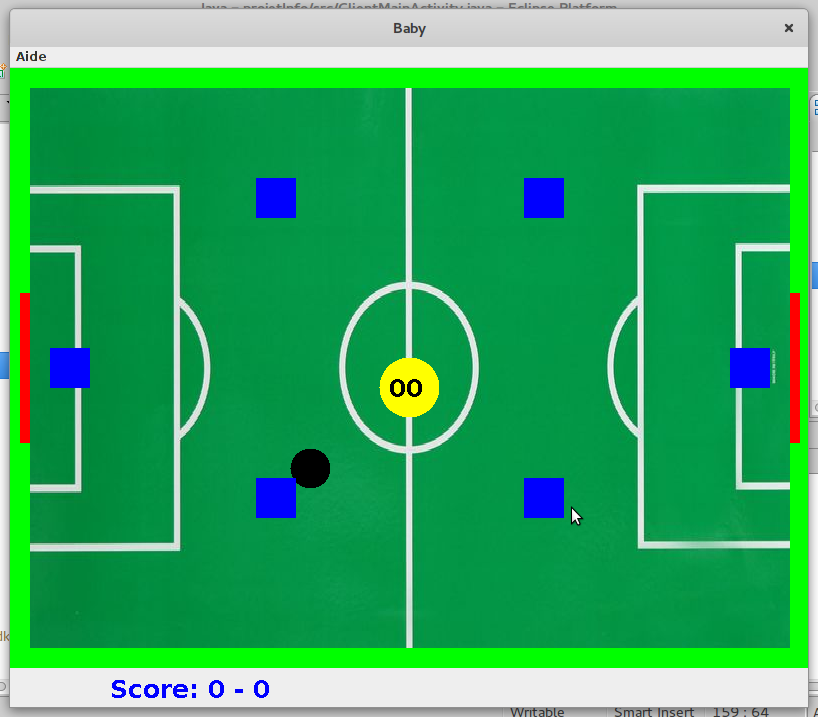
\includegraphics[width=15cm]{pictures/header.jpg}

\end{center}

\caption{Image d'accueil du programme, à la fois simple et efficace.}

\end{figure}

\paragraph{Commencer une partie}

Le jeu a été fait au plus simple, pour commencer une partie il suffit de lancer le programme en lui passant en paramètre, l'adresse IP du serveur. Il faut simplement que le serveur soit déjà lancé.

Une fois que les deux jours sont connectés, la partie commence automatiquement au bout de 10 secondes, permettant aux joueurs de se préparer, et de tester leurs commandes.




\paragraph{Déroulement d'une partie}

Le gameplay est entièrement manuel et voit le joueur maître de ses possibilités. Chaque Joueur contrôle deux lignes de joueurs, en angle et en hauteur, via une combinaison de touches. Chaque joueur, joue indépendamment sur son programme et essaie donc de marquer des buts. En cas de But, la balle repart au centre et on continue à jouer, un petit compteur permet aux joueurs de se préparer.




Dès que le score max est atteint, on affiche les scores. Et on déclare le vainqueur via des Popup.

\paragraph{Options}

Le jeu se veut simplifié au maximum, pour ne pas avoir de paramètres complexes à gérer, et ainsi pouvoir jouer directement. Il n'y a donc pas d'options, même si certains paramètres ont été codés pour être modifiés simplement, notamment, le nombre de buts qu'il faut inscrire pour gagner.

La seule chose dont il faut se préoccuper, c'est la précense d'un serveur, sinon le jeu refuse de démarrer.







%%%%%%%%%%%%%%%%%%%%%%%%%%%%%%%%%%

%% %%

%% ------------------------ %%

%% %%

%%%%%%%%%%%%%%%%%%%%%%%%%%%%%%%%%%

\chapter{Analyse de la solution envisagée et mise à jour}

%%%%%%%%%%%%%%%%%%%%%%%%%%%%%%%%%%

%% ------------------------ %%

%%%%%%%%%%%%%%%%%%%%%%%%%%%%%%%%%%

\section{Découpage en modules}

\paragraph{}

J'ai donc découpé le code en deux grandes parties :

\begin{itemize}

\item Partie client

\item Partie serveur

\end{itemize}

\begin{figure}[H]

\begin{center}

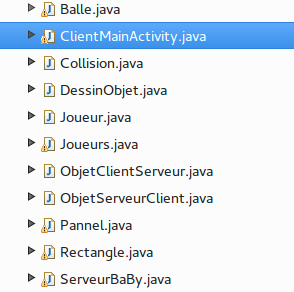
\includegraphics[width=07cm]{pictures/structure.png}

\end{center}

\caption{Structure des fichiers du projet.}

\end{figure}

Les deux parties (client/serveur) seront elles-mêmes séparées en plusieurs modules.

\begin{itemize}

\item L'interface graphique (rangée dans Pannel.java) qui sera utilisée sur le serveur seulement pour le débogage, mais qui consiste en une énorme part du client, et une des plus importantes.

\item La partie réseau de l'application (rangée dans les objets), qui forme les requêtes dans les deux sens.

\item Le c\oe{}ur algorithmique de l'application (rangée dans Collision.java) contenant les classes gérant c\oe{}ur du serveur qui se dans font l'ensemble des calculs du jeu.

\end{itemize}

Mais j'ai fait le choix, qu'une classe représente un objet ou une fonction, ainsi la classe balle, gère à la fois, la position de la balle, sa vitesse et son dessin, c'est donc cette classe qui est utilisée pour faire les collisions (c'est-à-dire passé en paramètre de la classe collision).

%%%%%%%%%%%%%%%%%%%%%%%%%%%%%%%%%%

%% ------------------------ %%

%%%%%%%%%%%%%%%%%%%%%%%%%%%%%%%%%%

\section{L'interface graphique (client)}

\paragraph{ClientMainActivity.java}

Gère la fenêtre qui englobe tout le reste. On utilisera en fait des JPanel pour modifier le contenu de cette fenêtre, dont celui défini dans Pannel. 

J'empêcherai dans un premier temps de modifier la taille de la fenêtre pour éviter d'avoir des problèmes de dessin du terrain de babyfoot à gérer.

Cette classe contient la \textbf{main} du programme. C'est elle qui lance le jeu et appelle le Jpannel

Cette classe a deux autres fonctions: la première c'est de cadencer le dessin du programme client, de scruter l'appui des touches, à 100hz, et de renvoyer tout cela au serveur via l'objet \emph{ObjetClientServeur.java}

Cette classe contient aussi une classe interne, héritant de Runnable, qui a pour objectif d'écouter le serveur à 200hz (c'est-à-dire que s’ il n'y a rien à écouter, on attend 5ms avant de recommencer) et de modifier en conséquence les attributs de la classe mère.

\paragraph{Panel.java}

Classe relativement simple, elle contient une liste d'objets dessinObjet, qu'elle initialise, puis dessine à l'appel de la fonction Main (elle est aussi utilisable sur le Serveur pour le débogage).




\paragraph{DessinObjet.java}

Classe abstraite définissant les méthodes communes à tous les objets destinés à être dessinés.

\begin{figure}[H]

\begin{center}

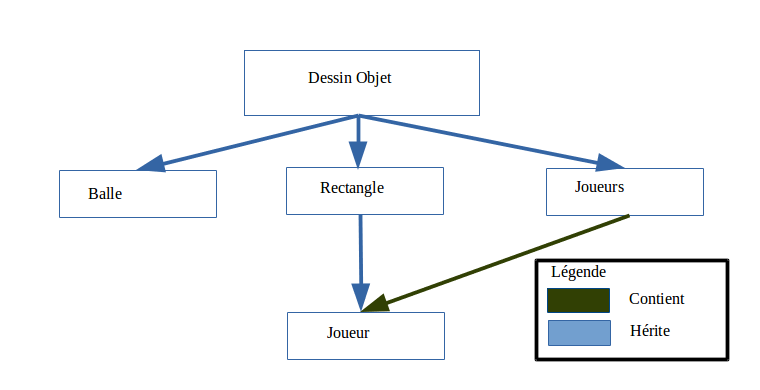
\includegraphics[width=17cm]{pictures/heritage.png}

\end{center}

\caption{Schéma des Structures d'héritage du projet.}

\end{figure}

Cette classe permet donc d'harmoniser les méthodes utilisées, et surtout de créer des listes d'objets qui se dessinent. Et ainsi être très souple sur ce qui doit être dessiné.

Elle implémente l'interface Sérialisable, on verra plus tard où cela est utilisé.

\paragraph{Balle.java}

Cette classe hérite donc de DessinObjet, elle contient la méthode pour dessiner la balle, ainsi que ses coordonnées, sa vitesse, sa couleur et son rayon. 

\paragraph{Rectangle.java}

C'est la même chose que la classe précédente, mais pour dessiner des Rectangles.

\paragraph{Joueur.java}

Hérite de Rectange, la seule différence est la manière de mettre à jour les coordonnées à partir des angles et de la hauteur des barres.

De plus ces rectangles ont deux modes, suivant l'angle, c'est-à-dire que si l'angle est supérieur (en valeur absolue) à 2*Pi/3, le Rectange devient gris, ce qui signifie, que le joueur à la tête en bas.

\paragraph{Joueurs.java}

La classe qui gère les joueurs, leur position initiale (c'est-à-dire défenseur, attaquant ...), mais aussi la gestion de la position de l'angle.

Elle a pour but de mettre à jour le tableau de (Joueur)s qu'elle contient avant de les dessiner.




%%%%%%%%%%%%%%%%%%%%%%%%%%%%%%%%%%

%% ------------------------ %%

%%%%%%%%%%%%%%%%%%%%%%%%%%%%%%%%%%

\section{Le réseau}

\subsection{Le principe général}

\paragraph{}

Des messages sont échangés entre le client et le serveur, et ce de façon répétée. Il faut donc utiliser des Thread pour gérer l'émission et la réception de données depuis le serveur et un Thread pour gérer la réception côté client. 

\subsection{La partie client}

\paragraph{ClientMainACtivity.java}

Dans cette classe, une classe interne s'occupe de lire les données reçues, et de les modifier dans la classe mère.

De plus à chaque dessin, on envoie les données actuelles au serveur ( c'est-à-dire la position des joueurs )

\subsection{La partie serveur}

\paragraph{ServerBaby.java}

Classe de base du Serveur, qui teste les collisions, gère les rebond, fait avancer la balle, et fait transiter les données, entre les clients et le serveur, c'est de loin la classe la plus complexe.

%%%%%%%%%%%%%%%%%%%%%%%%%%%%%%%%%%

%% ------------------------ %%

%%%%%%%%%%%%%%%%%%%%%%%%%%%%%%%%%%

\section{Le c\oe{}ur algorithmique}

\paragraph{ServeurBaBy.java}

Le c\oe{}r algorithmique du programme est le serveur, c'est lui qui gère le fonctionnement du programme. 

\lstinputlisting[language=Java, firstline=282, lastline=302]{../src/ServeurBaBy.java}

\lstinputlisting[language=Java, firstline=269, lastline=269]{../src/ServeurBaBy.java}

On voit sur cette fonction, qui représente la boucle du serveur, comment celui-ci fonctionne:

\begin{itemize}

\item On commence par déplacer la balle

\item On vérifie s’ il y a collision entre les buts et la balle.

\item ensuite, on liste tous les Réctangles(dont les joueurs, qui ont plusieurs \og{}Joueurs\fg) et on effectue les collisions

\item on effectue une petite pause.

\item on envoie les données de jeu

\end{itemize}




On donc ici quelques fonctions indépendantes.

\paragraph{deplacerBalle}




\lstinputlisting[language=Java, firstline=332, lastline=350]{../src/ServeurBaBy.java}

Ici aussi le fonctionnement est simple:

\begin{itemize}

\item on vérifie que la balle a une vitesse admissible, sinon on la modifie

\item On applique un genre de frottement solide de la forme: $ m \frac{\vec{dv}}{dt} = - f\vec{v} $ et en linéarisant au premier ordre, cela suffit pour un premier modèle.

\end{itemize}




\paragraph{Envoie des données}

\lstinputlisting[language=Java, firstline=148, lastline=165]{../src/ServeurBaBy.java}

Ici, on récupère les objets du Serveur, on les affecte à l'objet de transmission et on envoie.







\paragraph{Collision}

\lstinputlisting[language=Java, firstline=200, lastline=213]{../src/ServeurBaBy.java}

[..]

\lstinputlisting[language=Java, firstline=240, lastline=251]{../src/ServeurBaBy.java}

Le programme de Collsion est de loin le plus complexe à gérer, mais en voici le principe:

\begin{itemize}

\item On vérifie d'abord si les objets sont en collision, si c'est le cas on continue, cette fonction est relativement complexe et sera détaillée plus tard.

\item Si c'est le cas, on essaie de déterminer le type de collision, par exemple si la balle arrive par la droite sur un mur vertical :

\begin{figure}[H]

\begin{center}

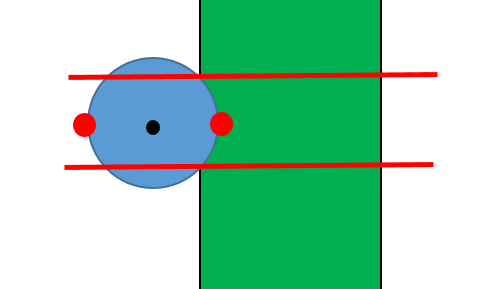
\includegraphics[width=8cm]{pictures/Capture.PNG}

\end{center}

\caption{Exemple de collision disque/rectangle}

\end{figure}

Comme c'est le cas sur la première condition du code:

\lstinputlisting[language=Java, firstline=207, lastline=209]{../src/ServeurBaBy.java}

On vérifie donc deux choses, le point rouge de droite est dans le mur, alors que celui de gauche n'y ait pas (attention, si l'on est rentré complètement dans le mur, il ne se passe rien, c'est la faiblesse de cet algorithme, même si en pratique, le cas ne se présente pas)

puis on vérifie qu'entre les deux lignes rouges, il y a du mur, par exemple sur la figure suivante, ce n'est pas le cas, donc on effectuera plutôt une collision de coin.

\begin{figure}[H]

\begin{center}

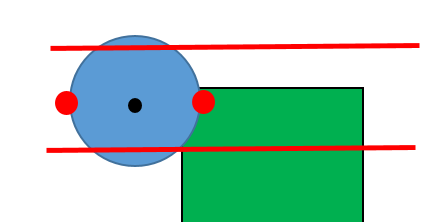
\includegraphics[width=8cm]{pictures/Capture2.PNG}

\end{center}

\caption{Exemple de collision disque/rectangle}

\end{figure}

\item si on rentre dans une des conditions, on inverse la vitesse concernée, sinon, on considère que c'est une collision de coin, car l'on sait qu'il y a collision.

\item

\lstinputlisting[language=Java, firstline=240, lastline=247]{../src/ServeurBaBy.java}

Enfin on considère que s’ il y a collision, elle est effectuée et donc on en fera pas d'autre tant que l'on n’a pas quitté le contacte, cela permet d'éviter d'avoir des balles qui n'arrivent pas à sortir des murs, pour cela, on procède comme cela:

\lstinputlisting[language=Java, firstline=240, lastline=247]{../src/ServeurBaBy.java}

à chaque contacte, on affecte une variable enContactAvecLaBalle à \emph{true}, et tant qu'il y aura collision, elle restera à \emph{true} ainsi, avant de faire une collision, on va la vérifier:

\lstinputlisting[language=Java, firstline=201, lastline=202]{../src/ServeurBaBy.java}

et si on n'a plus de collision, on désactive cette variable.




\end{itemize}




%%%%%%%%%%%%%%%%%%%%%%%%%%%%%%%%%%

%% %%

%% ------------------------ %%

%% %%

%%%%%%%%%%%%%%%%%%%%%%%%%%%%%%%%%%

\chapter{Échéancier}

\paragraph{ce qui était prévu}

\begin{enumerate}

\item \textbf{Fin décembre} : rédiger l'avant-projet.

\item \textbf{Début/Mi-Janvier} : obtenir la validation et les annotations sur la structure choisie.

\item \textbf{Fin janvier} : réaliser la partie graphique du programme et avoir regardé les grandes lignes du développement serveur. Avoir mis au point les éléments de base du gameplay (interaction joueur/machine).

\item \textbf{Fin février} : développer le serveur et la gestion des différents types de requêtes.

\item \textbf{Mi-Mars} : dresser les liens entre serveur et jeu. Tester.

\end{enumerate}

\paragraph{Ce qui a été fait}

\begin{enumerate}

\item \textbf{Fin décembre} : rédiger l'avant-projet.

\item \textbf{Fin décembre/Début janvier} : développer la partie réseau et l'architecture de base des requêtes.

\item \textbf{Fin janvier} : réalisation de l'interface graphique et des premiers calculs pour la mise en place de matchs.

\item \textbf{Février} : ajout des collisions et corrections des principaux bugs liés à la gestion des joueurs.

\item \textbf{Mars} : déboguer le reste du programme et ajouter les fonctionnalités supplémentaires nécessaires à un bon fonctionnement.

\end{enumerate}

\part{Évolutions vis-à-vis de l'avant-projet}

\begin{figure}[H]

\begin{center}

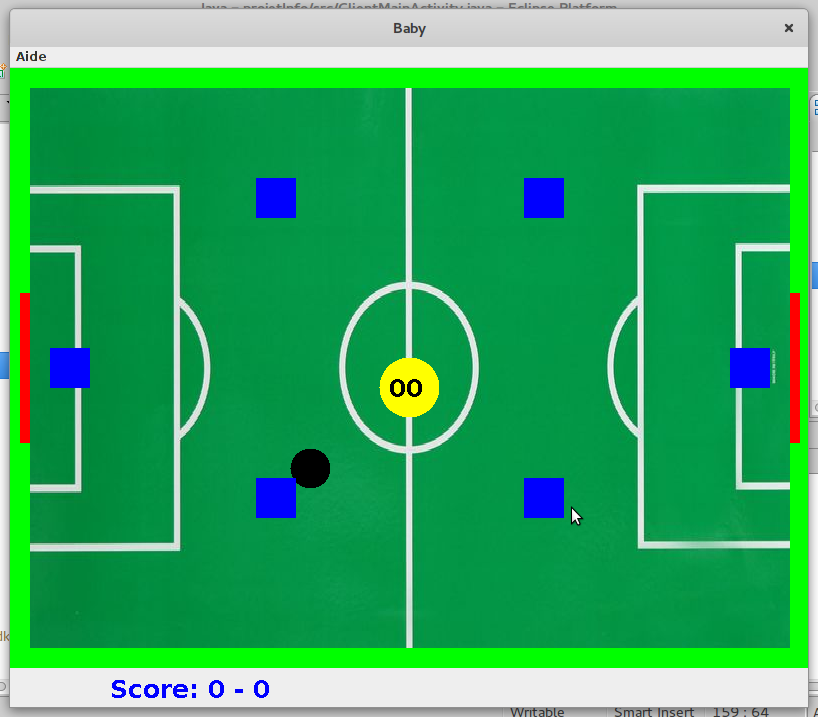
\includegraphics[width=15cm]{pictures/header.jpg}

\end{center}

\caption{Capture d'écran du jeu lui-même et de son aspect.}

\end{figure}

\paragraph{}

Le projet a été globalement mené à son terme bien qu'il subsiste de nombreux points à améliorer. La programmation de ce projet relativement ambitieux (quelques $3000$ lignes de code jusque là) m'a toutefois permis d'appréhender la mise en place d'un réseau en java et le dessin d'une interface graphique. Il aurait pu être intéressant, devant l'envergure que peut prendre un tel projet, de chercher à implanter une stratégie \emph{MVC}, modèle Vue Controleur, sur le client afin de faciliter l'édition de l'interface graphique et la gestion des données reçues du serveur. 

\paragraph{Pour ce qui est de la structure}

J'ai rajouté quelques classes au projet initial, mais toutes n'ont pas été mentionnées ci-dessus, car certaines ne sont parfois que des classes implantant l'interface Runnable et initiant des Thread. Globalement, la structure est restée la même, en séparant toutefois bien client et serveur néanmoins, afin de laisser la possibilité que le serveur soit lancé sur une machine indépendante tandis que le client est distribué.

\paragraph{Pour ce qui est du code}

Il y a relativement peu de commentaires sur l'ensemble du projet, car il y a très peu de points très techniques méritant une explication. Le plus difficile est de comprendre l'agencement des classes et leur hiérarchie dans la chaîne aboutissant au jeu.

\paragraph{Choix techniques}

J'ai bien sûr utilisé \textbf{Swing} pour réaliser l'interface graphique : d'abord pour la simple raison que le double-buffering est automatiquement utilisé par Swing, ensuite parce que la structure d'une fenêtre est beaucoup plus souple en ce qui concerne la réalisation de quelque chose d'un peu plus complet, même si je n'en ai pas eu besoin ici, mais dans une évolution future. En ce qui concerne le système réseau, j'ai tout simplement utilisé des sockets et des objets Sérialisés, ainsi qu'ils sont décrits dans le polycopié du cours d'informatique.

\part{Explications des choix techniques}

%%%%%%%%%%%%%%%%%%%%%%%%%%%%%%%%%%

%% ------------------------ %%

%%%%%%%%%%%%%%%%%%%%%%%%%%%%%%%%%%

\section{Le réseau}

\paragraph{}

Le réseau est au coeur de mon projet et j'ai donc développé plusieurs Thread en parallèle pour pouvoir gérer plus facilement l'envoi de messages par mon application.


\section{Algorithmique}

\paragraph{}

L'intervalle de temps entre l'envoi de la requête et la réception est aussi légèrement variable et est difficilement quantifiable puisque cela dépend de la charge de l'ordinateur et de l'utilisation du client au moment de la réception du message. Il m'a donc fallu faire patienter le client ou le faire utiliser des données \og périmées \fg.

\paragraph{}

L'utilisation d'objets Sérialisable pour transmettre les données, permets une très grande souplesse, car si l'on veut envoyer une information de plus au client ou au serveur, il suffit de rajouter un attribut à l'objet concerné, comme les demandes de pause:

\lstinputlisting[language=Java, firstline=4, lastline=13]{../src/ObjetServeurClient.java}

\paragraph{}

Pour calculer la position de la balle au cours du temps, j'ai utilisé un Thread qui s'actualise toutes les 10ms et qui effectue à chaque tour d'horloge comme présentée précédemment,

l'actualisation de la position à partir de la vitesse et des tests de collisions. Les tests de collisions sont calculés à part dans une classe appelée Collision.

\paragraph{}

La principale difficulté algorithmique vient de cet aspect justement. Parvenir à prévoir les différents comportements de la balle par rapport aux

joueurs. Les coordonnées utilisées par ces calculs diffèrent en plus parfois de celles d'affichage et il faut prendre en compte la taille de l'écran ainsi que les imprécisions dues au caractère discret du calcul. J'ai encore parfois des problèmes de collisions qui se produisent trop tôt, c'est-à-dire que le joueur humain a l'impression qu'elle se cogne contre un objet invisible, ou encore des collisions gérées trop tard auquel cas la balle rentre partiellement dans le joueur en plastique. Voir parfois des problèmes de balles qui traversent, à cause de l'hystérésis de collision (\emph{EnContacteAvecLaBalle} à true) et la vitesse qui ne s'inverse pas quand elle devrait.

\paragraph{}

Le problème des collisions est-ce qui m'a pris le plus de temps, et si j'ai déjà expliqué comment elles étaient utilisées, la partie détection est la plus complexe, car elle doit s'exécuter très rapidement. De plus si une intersection rectangle rectangle est simple, une intersection sphère rectangle est bien plus lourde en calcul. En effet de nombreux cas sont possibles:

\begin{figure}[H]

\begin{center}

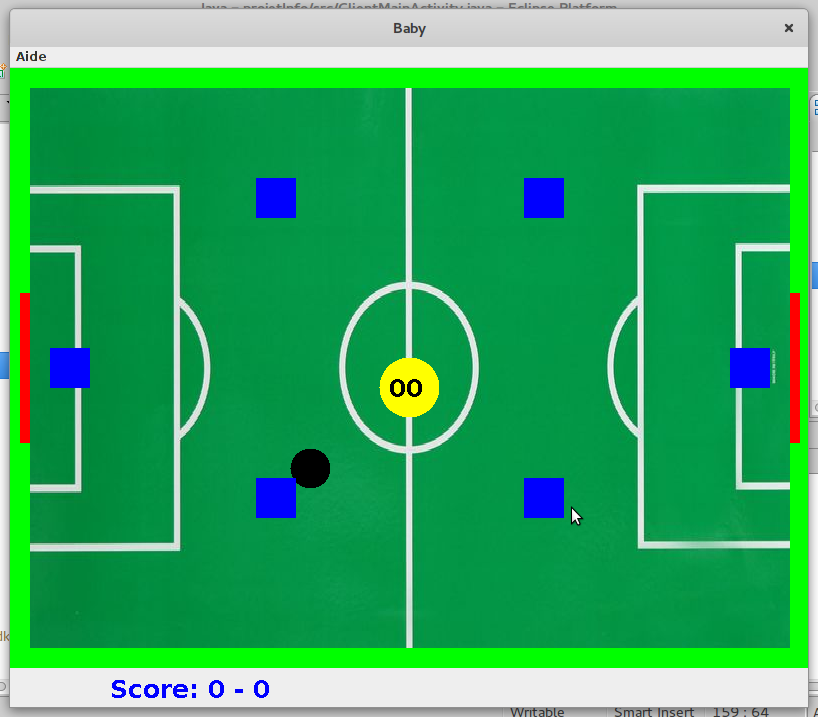
\includegraphics[width=15cm]{pictures/header.jpg}

\end{center}

\caption{Les différentes possibilités de collisions. Source:openclassrooms.com}

\end{figure}




Ici, j'ai supposé que les cas C et D n'étaient pas en envisagé, car ils ne doivent pas se produire, et de toute façon, ce ne sont pas les plus intéressants, ils se détectent aisément avec une collision rectangle/rectangle.

De plus j'ai commencé par vérifier la collision entre le rectangle et le rectangle entourant la balle.




ensuite il faut traiter de nombreux cas:

\lstinputlisting[language=Java, firstline=13, lastline=32]{../src/Collision.java}




\paragraph{}

Le problème du caractère discret de ces calculs, c'est que les corrections ne suffisent pas à faire sortir la balle de la zone de collision. Ainsi, malgré le changement de vitesse et la correction effectuée lorsque la balle entre dans une des zones où la collision a lieu, il est possible que la balle reste dans une de ces zones auquel cas, le prochain tour de calcul risque de demander un nouveau changement de vitesse ce qui est bien sûr absurde. D'où la nécessite d'une hystérésis présentée au-dessus.

\paragraph{}

J'ai essayé de mettre au point un amortissement de la vitesse de la balle au cours du jeu. Il est difficile de s'en occuper, car, en conservant quelque chose de significatif, il arrive que la balle s'immobilise ce qui est légèrement problématique. D'où l'idée d'apposer des bornes, mais cela n'est pas parfaite, le mieux aurait été de séparer vitesse et direction (une norme et un angle) et d'imposer des bornes à la vitesse, car là, la balle ne peut être verticale...

\definecolor{gray}{gray}{0.5}
\definecolor{green}{rgb}{0,0.5,0}
\lstloadlanguages{Java}
\lstset{language=Java}
\lstset{%
inputencoding=utf8,
extendedchars=true,
literate=%
{é}{{\'{e}}}1
{è}{{\`{e}}}1
{ê}{{\^{e}}}1
{ë}{{\¨{e}}}1
{û}{{\^{u}}}1
{ù}{{\`{u}}}1
{â}{{\^{a}}}1
{à}{{\`{a}}}1
{î}{{\^{i}}}1
{ô}{{\^{o}}}1
{ç}{{\c{c}}}1
{Ç}{{\c{C}}}1
{É}{{\'{E}}}1
{Ê}{{\^{E}}}1
{À}{{\`{A}}}1
{Â}{{\^{A}}}1
{Î}{{\^{I}}}1
}
\end{document} 



